% Template for PLoS
% Version 3.5 March 2018
%
% % % % % % % % % % % % % % % % % % % % % %
%
% -- IMPORTANT NOTE
%
% This template contains comments intended 
% to minimize problems and delays during our production 
% process. Please follow the template instructions
% whenever possible.
%
% % % % % % % % % % % % % % % % % % % % % % % 
%
% Once your paper is accepted for publication, 
% PLEASE REMOVE ALL TRACKED CHANGES in this file 
% and leave only the final text of your manuscript. 
% PLOS recommends the use of latexdiff to track changes during review, as this will help to maintain a clean tex file.
% Visit https://www.ctan.org/pkg/latexdiff?lang=en for info or contact us at latex@plos.org.
%
%
% There are no restrictions on package use within the LaTeX files except that 
% no packages listed in the template may be deleted.
%
% Please do not include colors or graphics in the text.
%
% The manuscript LaTeX source should be contained within a single file (do not use \input, \externaldocument, or similar commands).
%
% % % % % % % % % % % % % % % % % % % % % % %
%
% -- FIGURES AND TABLES
%
% Please include tables/figure captions directly after the paragraph where they are first cited in the text.
%
% DO NOT INCLUDE GRAPHICS IN YOUR MANUSCRIPT
% - Figures should be uploaded separately from your manuscript file. 
% - Figures generated using LaTeX should be extracted and removed from the PDF before submission. 
% - Figures containing multiple panels/subfigures must be combined into one image file before submission.
% For figure citations, please use "Fig" instead of "Figure".
% See http://journals.plos.org/plosone/s/figures for PLOS figure guidelines.
%
% Tables should be cell-based and may not contain:
% - spacing/line breaks within cells to alter layout or alignment
% - do not nest tabular environments (no tabular environments within tabular environments)
% - no graphics or colored text (cell background color/shading OK)
% See http://journals.plos.org/plosone/s/tables for table guidelines.
%
% For tables that exceed the width of the text column, use the adjustwidth environment as illustrated in the example table in text below.
%
% % % % % % % % % % % % % % % % % % % % % % % %
%
% -- EQUATIONS, MATH SYMBOLS, SUBSCRIPTS, AND SUPERSCRIPTS
%
% IMPORTANT
% Below are a few tips to help format your equations and other special characters according to our specifications. For more tips to help reduce the possibility of formatting errors during conversion, please see our LaTeX guidelines at http://journals.plos.org/plosone/s/latex
%
% For inline equations, please be sure to include all portions of an equation in the math environment.  For example, x$^2$ is incorrect; this should be formatted as $x^2$ (or $\mathrm{x}^2$ if the romanized font is desired).
%
% Do not include text that is not math in the math environment. For example, CO2 should be written as CO\textsubscript{2} instead of CO$_2$.
%
% Please add line breaks to long display equations when possible in order to fit size of the column. 
%
% For inline equations, please do not include punctuation (commas, etc) within the math environment unless this is part of the equation.
%
% When adding superscript or subscripts outside of brackets/braces, please group using {}.  For example, change "[U(D,E,\gamma)]^2" to "{[U(D,E,\gamma)]}^2". 
%
% Do not use \cal for caligraphic font.  Instead, use \mathcal{}
%
% % % % % % % % % % % % % % % % % % % % % % % % 
%
% Please contact latex@plos.org with any questions.
%
% % % % % % % % % % % % % % % % % % % % % % % %

\documentclass[10pt,letterpaper]{article}
\usepackage[top=0.85in,left=2.75in,footskip=0.75in]{geometry}

% amsmath and amssymb packages, useful for mathematical formulas and symbols
\usepackage{amsmath,amssymb}

% Use adjustwidth environment to exceed column width (see example table in text)
\usepackage{changepage}

% Use Unicode characters when possible
\usepackage[utf8x]{inputenc}

% textcomp package and marvosym package for additional characters
\usepackage{textcomp,marvosym}

% cite package, to clean up citations in the main text. Do not remove.
\usepackage{cite}

% Use nameref to cite supporting information files (see Supporting Information section for more info)
\usepackage{nameref,hyperref}

% line numbers
\usepackage[right]{lineno}

% ligatures disabled
\usepackage{microtype}
\DisableLigatures[f]{encoding = *, family = * }

% color can be used to apply background shading to table cells only
\usepackage[table]{xcolor}

% array package and thick rules for tables
\usepackage{array}

% create "+" rule type for thick vertical lines
\newcolumntype{+}{!{\vrule width 2pt}}

% create \thickcline for thick horizontal lines of variable length
\newlength\savedwidth
\newcommand\thickcline[1]{%
	\noalign{\global\savedwidth\arrayrulewidth\global\arrayrulewidth 2pt}%
	\cline{#1}%
	\noalign{\vskip\arrayrulewidth}%
	\noalign{\global\arrayrulewidth\savedwidth}%
}

% \thickhline command for thick horizontal lines that span the table
\newcommand\thickhline{\noalign{\global\savedwidth\arrayrulewidth\global\arrayrulewidth 2pt}%
	\hline
	\noalign{\global\arrayrulewidth\savedwidth}}


% Remove comment for double spacing
%\usepackage{setspace} 
%\doublespacing

% Text layout
\raggedright
\setlength{\parindent}{0.5cm}
\textwidth 5.25in 
\textheight 8.75in

% Bold the 'Figure #' in the caption and separate it from the title/caption with a period
% Captions will be left justified
\usepackage[aboveskip=1pt,labelfont=bf,labelsep=period,justification=raggedright,singlelinecheck=off]{caption}
\renewcommand{\figurename}{Fig}

% Use the PLoS provided BiBTeX style
\bibliographystyle{plos2015}

% Remove brackets from numbering in List of References
\makeatletter
\renewcommand{\@biblabel}[1]{\quad#1.}
\makeatother



% Header and Footer with logo
\usepackage{lastpage,fancyhdr,graphicx}
\usepackage{epstopdf}
%\pagestyle{myheadings}
\pagestyle{fancy}
\fancyhf{}
%\setlength{\headheight}{27.023pt}
%\lhead{\includegraphics[width=2.0in]{PLOS-submission.eps}}
\rfoot{\thepage/\pageref{LastPage}}
\renewcommand{\headrulewidth}{0pt}
\renewcommand{\footrule}{\hrule height 2pt \vspace{2mm}}
\fancyheadoffset[L]{2.25in}
\fancyfootoffset[L]{2.25in}
\lfoot{\today}

%% Include all macros below

\usepackage{refcount}
\usepackage{textgreek}
\usepackage{bm}

\newcommand{\unit}[1]{\,\mathrm{#1}}
\newcommand{\n}[1]{\mathrm{#1}}
\newcommand{\dd}[2]{\frac{\mathrm{d} #1}{\mathrm{d} #2}}
\newcommand*{\defeq}{\mathrel{\vcenter{\baselineskip0.5ex \lineskiplimit0pt
			\hbox{\scriptsize.}\hbox{\scriptsize.}}}%
	=}
\newcommand\subref[2]{%
	\def\myref{\getrefnumber{#1}}% extract the reference number
	\hyperref[#1]{\myref\mbox{#2}}% print the reference number with argument
}

\hyphenation{XapA}
\hyphenation{XapB}
\hyphenation{XapR}
\hyphenation{XapAB}
\hyphenation{XapABR}
\hyphenation{xapA}
\hyphenation{xapB}
\hyphenation{xapR}
\hyphenation{xapAB}
\hyphenation{xapABR}

\reversemarginpar

%% END MACROS SECTION


\begin{document}
	\vspace*{0.2in}
	
	% Title must be 250 characters or less.
	\begin{flushleft}
		{\Large
			\textbf\newline{Theoretical investigation of a genetic switch for metabolic adaptation} % Please use "sentence case" for title and headings (capitalize only the first word in a title (or heading), the first word in a subtitle (or subheading), and any proper nouns).
		}
		\newline
		% Insert author names, affiliations and corresponding author email (do not include titles, positions, or degrees).
		\\
		Kathrin S. Laxhuber\textsuperscript{1},
		Muir J. Morrison\textsuperscript{2},
		Griffin Chure\textsuperscript{3},
		Rob Phillips\textsuperscript{2,3$\ast$}
		\\
		\bigskip
		\textbf{1} Department of Chemistry and Applied Biosciences, ETH Zurich, 8093 Zurich, Switzerland
		\\
		\textbf{2} Department of Physics, California Institute of Technology, Pasadena, CA, USA
		\\
		\textbf{3} Division of Biology and Biological Engineering, California Institute of Technology, Pasadena, CA, USA
		\\
		\bigskip
		
		% Insert additional author notes using the symbols described below. Insert symbol callouts after author names as necessary.
		% 
		% Remove or comment out the author notes below if they aren't used.
		%
		% Primary Equal Contribution Note
		% Yinyang These authors contributed equally to this work.
		
		% Additional Equal Contribution Note
		% Also use this double-dagger symbol for special authorship notes, such as senior authorship.
		% \ddag These authors also contributed equally to this work.
		
		% Current address notes
		% \textcurrency Current Address: Dept/Program/Center, Institution Name, City, State, Country % change symbol to "\textcurrency a" if more than one current address note
		% \textcurrency b Insert second current address 
		% \textcurrency c Insert third current address
		
		% Use the asterisk to denote corresponding authorship and provide email address in note below.
		$\ast$ phillips@pboc.caltech.edu
		
	\end{flushleft}
	% Please keep the abstract below 300 words
	\section*{Abstract}
	Membrane transporters carry key metabolites across the cell membrane
	and, from a resource standpoint, are hypothesized to be produced when necessary. The
	expression of membrane transporters in metabolic pathways is often
	upregulated by the transporter substrate. In \emph{E. coli}, such systems
	include for example the \emph{lacY}, \emph{araFGH}, and \emph{xylFGH} genes,
	which encode for lactose, arabinose, and xylose transporters, respectively.
	As a case study of a minimal system, we build a
	generalizable physical model of the \emph{xapABR} genetic
	circuit, which features a regulatory feedback loop via membrane
	transport (positive feedback) and enzymatic degradation (negative feedback)
	of an inducer. Dynamical systems analysis and stochastic simulations show
	that the membrane transport makes the model system bistable in certain
	parameter regimes. Thus, it serves as a genetic ``on-off'' switch, enabling
	the cell to only produce a set of metabolic enzymes when the corresponding
	metabolite is present in large amounts. We find that the negative feedback
	from the degradation enzyme does not significantly disturb the positive
	feedback from the membrane transporter. We investigate hysteresis in the
	switching and discuss the role of cooperativity and multiple binding sites
	in the model circuit. Fundamentally, this work explores how a stable genetic
	switch for a set of enzymes is obtained from transcriptional auto-activation
	of a membrane transporter through its substrate.
	
	\linenumbers
	
	% Use "Eq" instead of "Equation" for equation citations.
	% For figure citations, please use "Fig" instead of "Figure".
	% Place figure captions after the first paragraph in which they are cited.
	% Results and Discussion can be combined.
	% Place tables after the first paragraph in which they are cited.
	% PLOS does not support heading levels beyond the 3rd (no 4th level headings).
	% Include only the SI item label in the paragraph heading. Use the \nameref{label} command to cite SI items in the text.
	
	\section*{Introduction} 
	Genetic regulatory circuits are fundamental building blocks of functioning
	cells and organisms. One abundant class of these circuits are genetic
	switches. Although their construction and function may differ,
	their common feature is bistability: their output gene expression
	will flow to and remain at one of two steady-state levels.
	The distribution of
	gene expression in a cell culture can then be bimodal. This is not to be
	confused with mere stochastic bimodality, where the system is not stable,
	and the gene expression in each cell can fluctuate between the two levels.
	
	One classic example of a genetic switch is a system where two repressor
	proteins each regulate the transcription of the
	other~\cite{Jacob1961,Gardner2000} (illustrated schematically in
	Fig~\ref{fig0:switches}). Here, one stable state is high expression of
	the first protein and low expression of the second,
	and the second stable state is the opposite. This
	switch enables the system to have a memory: if something induces expression
	of either one of the proteins, the system will remain in this state until a
	significant perturbation occurs. Another well-known and even simpler example
	is an auto-activating circuit in which a protein activates its own
	transcription~\cite{Wolf1998}. This gives the system an ``on-off'' switch.
	
	\begin{figure}%[h!]
		\centering
		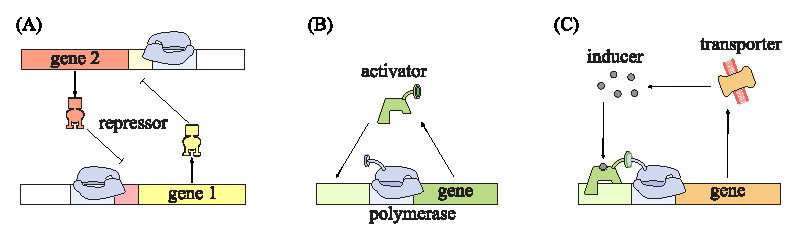
\includegraphics{media/Fig0_switches.eps}
		\caption{{\bf A schematic of different genetic switches.}
			(A) and (B) show the two most well-known genetic switches:
			(A) two mutual repressors and (B) a self-activating gene.
			In (C), a very much simplified version of the
			circuit that we investigate in this paper can be seen, where the
			similarity to the switch in (B) is clear. A complete version of
			the model circuit can be found in Fig~\ref{fig2:model}.}
		\label{fig0:switches}
	\end{figure}
	
	Through physical and mathematical modeling, we investigate a more complex
	switch system where the bistability is due, as we will show, to a
	membrane transport protein. Such a switch is common for
	metabolic processes in biology, for reasons discussed below.
	Existing models in the literature tend towards one of two extremes:
	either highly detailed descriptions of specific, complicated networks (e.g.,~\cite{Wong1997}),
	or Hill function descriptions that coarse-grain all complexity
	into a few parameters with inscrutable microscopic physical meaning.
	We aim for a middle ground in this work.
	We seek an intuitive understanding through a simple model of a minimal system,
	with only the essential components and interactions for the questions we pose.
	Yet we still model these components explicitly and
	discuss the necessary model complexity for a physically correct model.
	
	The key feature of the type of system we investigate is the indirect activation of
	the transporter gene by the transporter substrate, leading to positive
	feedback similar to the aforementioned ``on-off'' switch. An example for
	such an architecture is the \emph{lac} operon, where lactose indirectly
	activates the expression of lactose permease. Other examples in \emph{E.
		coli} include the \emph{araFGH} and \emph{xylFGH} operons, which contain genes for
	arabinose and xylose transporters, respectively. For \emph{lac} and
	\emph{araFGH}, bistability has indeed been observed and attributed to such a
	positive feedback
	loop, for example in the well-known study by Novick and Weiner (1957),
	among other works~\cite{Novick1957,Santillan2008,Ozbudak2004,Narang2008,Choi2008,Fritz2014,Jenkins2017,Siegele1997}.
	A eukaryotic example is the glucose transporter GLUT-2 in liver and
	\textbeta-cells~\cite{Bae2010,Tiedge1991}, though this system is much more
	complex than the following analysis.
	
	It is quite conceivable that this auto-activation process is common to many
	substances that a cell would want to consume. Such a switch enables the
	cell to sense and respond to its environment: if the substrate enters the
	cell, it activates the production of membrane transporters. The cell then
	starts accumulating the substrate, thereby ``testing'' the substrate's
	presence in the extracellular environment. If there is enough, the
	expression stabilizes at an ``on'' state and the cell has, in a short-term
	sense, adapted. When there is not enough substrate, the operon, which
	often encodes for a whole set of enzymes for this one metabolite, switches
	``off'' again. Such a mechanism could be involved in various cases of
	short-term adaptation.
	
	A key element of this mechanism is the presence of a transcription factor
	which binds to the transporter substrate and which is often expressed at a low level (often at copy numbers
	of order $\sim10$, \cite{Schmidt2015, Li2014}).
	This is resource efficient for the cell, as this low copy number
	transcription factor acts as an ``always on'' sensor to detect
	the substrate, allowing high copy numbers of the membrane transporter
	and its attendant operon to be expressed only when
	their substrate is actually present. The transcription factors
	LacI, AraC, and XylR all appear to fill this
	role~\cite{Novick1957,Santillan2008,Ozbudak2004,Narang2008,Choi2008,Fritz2014,Jenkins2017,Siegele1997,Song1997,Schmidt2015}.
	
	For our modeling, we focus on the \emph{xapABR} genetic circuit from
	\emph{E. coli} as a case study. It is similar to \emph{lac}, but less
	complex. Instead of lactose, its purpose is to make use of the nucleoside
	xanthosine as an energy source~\cite{Buxton1980,Hammer-Jespersen1980}. The
	circuit is made up of two operons: one that encodes for XapR and another
	that encodes for XapA and XapB. XapR is a transcription factor
	that is induced by xanthosine and activates the \emph{xapAB} promoter,
	in close analogy to AraC, XylR, and also LacI.\footnote{One might object that LacI represses its target operon, while
	XapR, AraC, and XylR activate their target operons. However, the analogy
	we wish to draw is that the qualitative logic of their inducers are all
	identical, i.e., the presence of their respective inducer causes their
	target operon to be transcribed.} The \textit{xapAB} promoter has been suggested to have two binding sites for XapR\cite{Seeger1995},
	but the promoter architecture and function is not yet fully understood. The
	transcription of \emph{xapR} seems to be constitutive and not
	auto-regulated~\cite{Seeger1995}. Structural homology to other transcription
	factors suggests that XapR appears in dimers where one dimer can bind two
	xanthosine molecules~\cite{Joergensen1999}. The protein XapA is a purine
	nucleoside phosphorylase that degrades xanthosine into components (ribose
	and xanthine) that can be fed into metabolic
	pathways~\cite{Buxton1980,Hammer-Jespersen1980}. XapB on the other hand is a
	membrane transporter of xanthosine~\cite{Seeger1995,Norholm2001}.
	
	Experimentally, we found that the expression level of \emph{xapAB} among
	cells is bimodal and that the system seems to be
	bistable (see next section). We aim to understand which of the circuit's
	features are necessary for bistability and investigate its behavior in
	different parameter regimes. After presenting some experimental background on the \emph{xap} genes, we discuss the
	details of our model. Next, we estimate the free parameters and then present
	the observations we made through phase diagrams, followed by the results
	from stochastic simulations.
	
	\section*{Experimental motivation} \label{sec:experiment}
	Our work was motivated by the experimental observation of bimodality
	in the \emph{xap} circuit, which is shown in Fig~\ref{fig1:data}. We
	focus on the essential findings here and refer the reader
	to~\nameref{S1_Text} for more experimental details. Briefly, we
	placed a fluorescent reporter under the control of the wild type
	(wt) \emph{xapAB} promoter. This construct was placed in three
	different backgrounds: \textDelta\emph{xapABR},
	\textDelta\emph{xapAB}, and wt,
	and expression as a function of extracellular xanthosine concentration
	was measured using flow cytometetry, as has been described
	previously~\cite{RazoMejia2018}. The left panel of
	Fig~\subref{fig1:data}{A} shows that for increasing xanthosine
	concentration, expression in the wt-background increases in a
	switch-like way: it is nearly zero when there is little xanthosine
	(``uninduced state''), but increases drastically when there is more
	(``induced state''). In between, the aforementioned bimodal
	distribution is obtained, where some bacteria are in the uninduced
	expression state and others are induced.
		
	\begin{figure}%[h!]
		\centering
		\includegraphics[width=1\textwidth]{media/Fig1_experiment.eps}
		\caption{{\bf Experimental data on the \emph{xap} circuit.}
		(A) The expression of the \emph{xapAB} promoter was measured for
		different extracellular concentrations of xanthosine (vertical axis).
		The left panel shows the wild type circuit while
		the middle and right panels show the effect of deleting
		the genes \emph{xapABR} and \emph{xapAB}, respectively.
		The wild type circuit behaves like a
		switch. Note that the fluorescence scale of the middle panel
		is not comparable with the other two,
		and also that the chosen xanthosine concentrations are different.
		(B) shows the fold-change in gene expression upon addition of
		xanthosine for the wt promoter (left panel)
		and for the promoter with only the XapR binding site adjacent
		to the polymerase binding site (right panel).
		Note that the fold-change used here differs from fold-change in,
		e.g.,~\cite{Garcia2011,RazoMejia2018,Chure2019},
		in that no subtraction of autofluorescence was performed,
		which is adequate for the qualitative comparison
		of these two promoters.
		}
		\label{fig1:data}
	\end{figure}

	When all genes of the \emph{xapABR} circuit are removed, the
	xanthosine response of our reporter construct disappears (see
	Fig~\subref{fig1:data}{A}, left panel).
	This is the result of removing the transcription factor XapR that is
	induced by xanthosine. When only the genes \emph{xapAB} are removed
	but \emph{xapR} is kept, a response to the xanthosine concentration
	is regained but it is no longer switch-like (see
	Fig~\subref{fig1:data}{A}, middle panel). Instead, the distribution remains
	unimodal and simply shifts to higher expression as the xanthosine
	concentration is increased. As we will see later on, this is because
	the circuit now lacks the positive feedback loop due to the
	xanthosine membrane transporter XapB. 
	
	As mentioned in
	the introduction, there are two binding sites for XapR on the
	\emph{xapAB} promoter: one directly at the polymerase binding site
	and one further upstream.
	Working in the \textDelta\emph{xapAB} background,
	we measured the expression level of our reporter when driven by two
	constructs: the wild-type \emph{xapAB} promoter
	(Fig~\subref{fig1:data}{B}, left panel), and the \emph{xapAB}
	promoter with the upstream binding site removed
	(Fig~\subref{fig1:data}{B}, right panel).
	Clearly, removing one XapR binding site dramatically reduced the
	responsiveness of the promoter to xanthosine (though not apparent
	from Fig~\subref{fig1:data}{B}, this response remains detectable).
	
	Already, we believe these data, combined with the prior knowledge of
	the field, clearly suggest a minimal model of the \emph{xapABR}
	system. The construction and exploration of this model occupies the
	remainder of this work. We leave it for future work to
	quantitatively dissect and test the model, in the manner
	of~\cite{Garcia2011,RazoMejia2018,Chure2019}, for example.
	
	\section*{Model}
	\subsection*{Step by step modeling of the system}
	In this section, we present our model of the \emph{xapAB} genetic circuit.
	Fig~\ref{fig2:model} shows an overview of this model.
	The qualitative picture of the circuit switching its state is as follows:
	\begin{itemize}
		\item In the initial absense of XapB, small amounts of xanthosine permeate
				into and out of the cell (discussed in more detail below).
		\item The presence of xanthosine shifts XapR's equilibrium from inactive to active.
		\item Active XapR binds to the \emph{xapAB} promoter, leading to transcription.
		\item From this mRNA transcript, translation produces the two proteins XapA and XapB.
		\item XapB actively transports much larger amounts of xanthosine into the cell and XapA degrades xanthosine.
		\item Production of more XapA and XapB is balanced by degradation or dilution through cell divisions.
	\end{itemize}
	Because xanthosine activates the transcription factor XapR, we have positive
	and negative feedback loops due to XapB and XapA, respectively. The remainder
	of this subsection discusses each of the above steps in detail, leading us
	to a set of two coupled ODEs. More in-depth explanations can be found
	in~\nameref{S1_Text}.
	
	\begin{figure}%[h!]
		\centering
		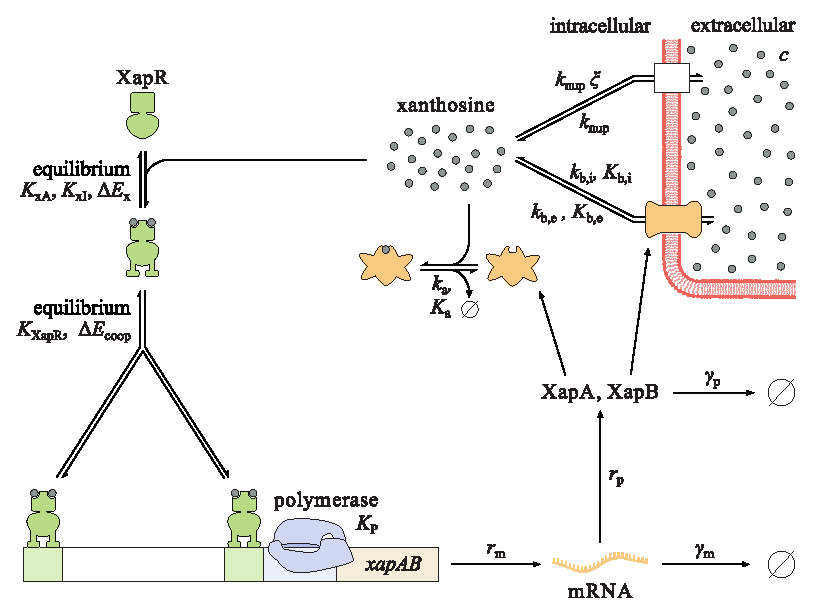
\includegraphics{media/Fig2_model.eps}
		\caption{{\bf Model of the \emph{xapAB} circuit.}
			The XapR dimers are induced by xanthosine and the induced XapR binds
			cooperatively as an activator to the \emph{xapAB} promoter. For
			these two steps, quasi-equilibrium is assumed. If both XapR binding
			sites are occupied and the polymerase is bound, the gene is
			transcribed at rate $r_{\n{m}}$. The mRNA decays at rate
			$\gamma_{\n{m}}$, and both proteins are translated at rate
			$r_{\n{p}}$ and decay at rate $\gamma_{\n{p}}$. XapA degrades
			xanthosine with Michaelis-Menten parameters $k_{\n{a}}$ and $K_{\n{a}}$.
			Similarly, XapB is treated as a Michaelis-Menten enzyme which imports ($k_{\n{b,i}}, K_{\n{b,i}}$) and exports ($k_{\n{b,e}}, K_{\n{b,e}}$) xanthosine. Furthermore, xanthosine enters and leaves the cell
			through non-specific transport, proportional to rates $k_{\n{nup}}$ and $\xi
			k_{\n{nup}}$, respectively.}
		\label{fig2:model}
	\end{figure}
	
	\paragraph*{Induction of XapR.} 
	We treat dimers as the only form of XapR that appears in the cell. Each
	dimer can bind two xanthosine molecules~\cite{Joergensen1999}. The Monod-Wyman-Changeux (MWC)
	model is used to describe the fraction of XapR dimers in the active state,
	which has the form
	\begin{eqnarray}
	\label{eq:MWC}
	\n{[XapR]_A} = \n{[XapR]_{tot}} \frac{\left(1 + \frac{\n{[x]}}{K_{\n{xA}}}\right)^2}{\left(1 + \frac{\n{[x]}}{K_{\n{xA}}}\right)^2 + e^{\beta \Delta E_{\n{x}}} \left(1+\frac{\n{[x]}}{K_{\n{xA}}} \frac{K_{\n{xA}}}{K_{\n{xI}}}\right)^2}.
	\end{eqnarray}
	A detailed discussion of the
	MWC model can be found in~\cite{Marzen2013}. In Eq~\ref{eq:MWC},
	$\n{[x]}$ is the xanthosine concentration, and $\n{[XapR]_A}$ and
	$\n{[XapR]_{tot}}$ denote the concentration of active and total XapR dimers,
	respectively. Furthermore, $K_{\n{xI}}$ and $K_{\n{xA}}$ are the
	dissociation constants of xanthosine to the inactive and the active XapR
	dimer, respectively, and $\Delta E_{\n{x}}$ stands for the energy difference
	between the inactive and the active states of the protein. We expect $\Delta E_{\n{x}} > 0$
	and $K_{\n{xA}} < K_{\n{xI}}$ for inducible activation. This corresponds to
	XapR being mainly inactive in the absence of xanthosine and becoming mostly
	active at high concentrations of xanthosine. 
	
	\paragraph*{Transcription.}
	Transcription and translation of the \emph{xapAB} gene, regulated by the
	induced XapR, produce the two proteins XapA and XapB. We start with
	transcription and assume that the binding of XapR and polymerase to the
	promoter is at quasi-equilibrium. The polymerase binding is modeled as
	independent of that of XapR, and all influence of the activator is pushed
	into the transcription rate. Furthermore, the binding energy of XapR to each
	of its two sites is assumed to be the same. A discussion of these
	simplifications can be found in~\nameref{S1_Text}.
	
	In Fig~\ref{fig3:states}, all possible states of the promoter in our model
	and their corresponding thermodynamic weights are shown. $\n{[P]}$
	denotes the polymerase concentration, and $\Delta E_{\n{coop}}$ stands for
	the interaction energy of the two XapR dimers. If cooperativity in
	transcription factor binding is neglected, this is set to zero. Furthermore,
	$K_{\n{XapR}}$ and $K_{\n{P}}$ denote the dissociation constant of XapR and
	polymerase to the promoter, respectively. In statistical mechanics language
	these dissociation constants are equivalent to
	$\frac{N_{\n{NS}}}{V} e^{\beta \Delta E_{\n{XapR}}}$
	and $\frac{N_{\n{NS}}}{V} e^{\beta \Delta E_{\n{P}}}$, respectively,
	with $N_{\mathrm{NS}}$ being the number of non-specific binding sites on the
	DNA, $V$ the volume of the cell, and $\Delta E_{\n{XapR}}$ and
	$\Delta E_{\n{XapR}}$, respectively, the interaction energies
	of XapR or polymerase with the promoter.
	
	\begin{figure}%[h!]
		\centering
		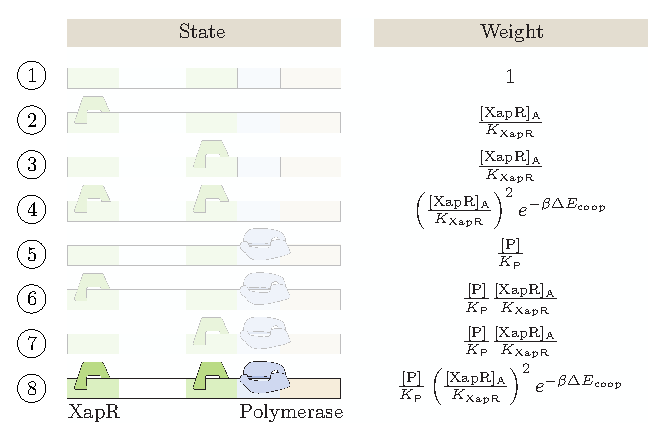
\includegraphics{media/Fig3_states.eps}
		\caption{{\bf The promoter states.} We consider only the completely
			occupied state as active and all other states (faded out in the figure)
			as completely inactive. The parameters are the interaction energy of
			the two XapR dimers $\Delta E_{\n{coop}}$ and the dissociation
			constants $K_{\n{XapR}}$ and $K_{\n{P}}$ of XapR and polymerase
			to the promoter, respectively. The concentrations of polymerase
			and active XapR are denoted by $\n{[P]}$ and $\n{[XapR]}$.}
		\label{fig3:states}
	\end{figure}
	
	We consider only the state where both XapR binding sites are occupied as
	active and all other states as inactive, meaning they have transcription
	rate equal to zero. Our experiments show that the expression becomes very weak when one of
	the XapR binding sites is removed from the promoter (see
	Fig~\subref{fig1:data}{B} and~\nameref{S1_Text}), suggesting that
	this simplification is reasonable. Furthermore, we find that in
	the bistable parameter range, considering the single occupancy states as
	active instead has almost no influence on the results (see
	also~\nameref{S1_Text}).
	
	With $\n{[m]}$ being the mRNA concentration, $r_{\n{m}}$ the transcription
	rate, $\gamma_{\n{m}}$ the mRNA decay rate, and $p_{\n{active}}$ the
	probability of the promoter being in the active state, we obtain
	\begin{eqnarray}
	\label{eq:mbasic}
	\dd{\n{[m]}}{t} &=& r_{\n{m}} p_{\n{active}} - \gamma_{\n{m}} \n{[m]} \\
	p_{\n{active}} &=& \frac{w_8}{\sum_{i=1}^{8} w_i} = 
	\frac{\n{[P]}}{K_{\n{P}}+\n{[P]}} 
	\frac{
		\left( \frac{\mathrm{[XapR]_A}}{K_{\mathrm{XapR}}} \right)^2 
		e^{- \beta \Delta E_{\n{coop}}}
	}{
		1 + 
		2 \frac{\mathrm{[XapR]_A}}{K_{\mathrm{XapR}}} +
		\left( \frac{\mathrm{[XapR]_A}}{K_{\mathrm{XapR}}} \right)^2 e^{- \beta \Delta E_{\n{coop}}}
	}
	\end{eqnarray}
	Here, $w_i$ stands for the thermodynamic weight of the ith state in the
	order in which they are listed in Fig~\ref{fig3:states}. As written above,
	the partition function factorizes into a polymerase and a XapR term because
	of our assumption of independent binding, which is further discussed
	in~\nameref{S1_Text}. Note that because $r_{\n{m}}$ implicitly contains the
	gene copy number per cell, it has units of $\n{M^{-1} \ s^{-1}}$ and not
	just $\n{s^{-1}}$. This rate equation gives the mean mRNA concentration
	$\langle\n{[mRNA]}\rangle = \frac{r_{\n{m}}}{\gamma_{\n{m}}}
	p_{\n{active}}$, which we will need in the next paragraph. The mean can also be found from the full chemical master equation, which is provided in~\nameref{S1_Text}.
	
	\paragraph*{Translation.} 
	The next step in our modeling progression is translation. As a
	simplification, we write $\n{[p]}=\n{[XapA]=[XapB]}$ for the general protein
	concentration. This assumes that the rates of transcription, mRNA decay,
	translation, and protein decay are the same for both proteins, which, as
	discussed in \nameref{S1_Text}, does not have a significant influence on the
	results. We write the following rate equation for the protein concentration,
	where $r_{\n{p}}$ denotes the translation rate, $\gamma_{\n{p}}$ the protein
	decay rate, and $\langle \n{[m]} \rangle$ the mean mRNA concentration:
	\begin{eqnarray}
	\label{eq:pbasic}
	\dd{\n{[p]}}{t} = r_{\n{p}} \langle \n{[m]} \rangle - \gamma_{\n{p}} \n{[p]}.
	\end{eqnarray}
	
	\paragraph*{Xanthosine dynamics.}
	Having described how xanthosine activates the synthesis of XapA and
	XapB through XapR, we now close the feedback loop
	by setting up a xanthosine rate equation.
	
	There are two significant mechanisms for transport of xanthosine across
	the cell membrane. In the induced system, the main transporter is XapB,
	whereas in the uninduced system, there is almost no XapB. Instead,
	xanthosine can enter the cell through the two nucleoside transporters
	NupC and NupG, which have a very low affinity for
	xanthosine~\cite{Norholm2001}. All these transporters, XapB, NupC, and
	NupG, are powered by the proton gradient across the
	membrane~\cite{Norholm2001}, which is why we assume their kinetic scheme
	to be similar to that of the \emph{lac} permease (as it is described
	in~\cite{Kaback2015}). There can be import and export of xanthosine, and
	which one dominates depends on the proton and xanthosine concentrations
	on the two sides of the membrane. In both cases, a proton and a
	substrate need to bind to the transporter on one side of the membrane
	and detach from it on the other side before the empty transporter moves
	back to the other side again. We refer the reader to~\nameref{S1_Text}
	for a detailed description of the transport and its modeling, and just
	state the result here. We model influx and efflux separately. For XapB,
	we use Michaelis-Menten kinetics with parameters $k_{\n{b, i}}$,
	$K_{\n{b, i}}$ for influx and $k_{\n{b, e}}, K_{\n{b,e}}$ for efflux.
	For the Nup transporters, we also use Michaelis-Menten kinetics but,
	because of the transporter's low affinity for xanthosine,
	we can linearize the Michaelis-Menten term as
	$k_{\n{cat}} {\n{[x]}}/(K_{\n{M}} + \n{[x]}) \approx \tilde{k} \n{[x]}$
	(i.e., $K_{\n{M}}~\gg~\n{[x]}$ across the physiologically relevant range for $\n{[x]}$).
	For the rate parameters $\tilde{k}$, we write $k_{\n{nup}}$ for
	influx and $\xi k_{\n{nup}}$ for efflux. 
		
	After transport into the cell, XapA degrades xanthosine. We model this using
	standard Michaelis-Menten kinetics, with parameters $k_{\n{a}}, K_{\n{a}}$
	(corresponding to turnover rate and Michaelis constant, respectively). Transport and degradation then leads to the xanthosine rate equation
	\begin{eqnarray}
	\dd{\n{[x]}}{t} = \biggl(\underbrace{k_{\n{b,i}} \frac{c}{K_{\n{b,i}} + c} - k_{\n{b,e}} \frac{\n{[x]}}{K_{\n{b,e}} + \n{[x]}}}_{\n{XapB}} - \underbrace{k_{\n{a}} \frac{\n{[x]}}{K_{\n{a}} + \n{[x]}}}_{\n{XapA}}\biggr) \n{[p]} + \underbrace{k_{\n{nup}} \left(c- \xi \n{[x]}\right)}_{\n{NupC\ \& \ NupG}}.
	\end{eqnarray}
	Recall that $\n{[x]}$ is the intracellular xanthosine concentration, while
	$c$ denotes the extracellular concentration. Because $k_{\n{b,i}} > k_{\n{b,e}}$ and
	$K_{\n{b,i}} < K_{\n{b,e}}$, influx dominates at low intracellular
	xanthosine concentrations. At much higher intra- than extracellular
	xanthosine concentrations, the efflux term takes over. More details on the
	aforementioned steps and a discussion of passive diffusion can be found
	in~\nameref{S1_Text}.
	
	\subsection*{Nondimensionalization}
	We have now formulated the behavior of the system in terms of the rate
	equations for mRNA, protein, and xanthosine. These equations can be
	nondimensionalized, which reduces the dimension of parameter space. We
	measure time in units of $\gamma_{\n{p}}^{-1}$ and concentrations in units
	of $K_{\n{a}}$ (except XapR, where the equations make it more natural to use
	$K_{\n{XapR}}$). In Table~\ref{table1:nondim}, all the nondimensional
	parameters and their definitions are listed. Furthermore, we define
	$\n{[m]_a} \defeq \frac{\n{[m]}}{K_{\n{a}}}$, $\n{[p]_a} \defeq
	\frac{\n{[p]}}{K_{\n{a}}}$, $\n{[x]_a} \defeq \frac{\n{[x]}}{K_{\n{a}}}$,
	and $\tau \defeq \gamma_{\n{p}} t$. Using these definitions, the following
	equations are obtained
	\begin{alignat}{2}
	\dd{\mathrm{[m]_a}}{\tau} &= \ &&
	\rho_{\n{m}} 
	\frac{
		\mathrm{[XapR]_{R,A}}^2 
		e^{- \Delta \epsilon_{\text{coop}}}
	}{
		1 + 
		2 \mathrm{[XapR]_{R,A}} +
		\mathrm{[XapR]_{R,A}}^2 e^{- \Delta \epsilon_{\text{coop}}}
	}
	- \gamma_{\n{mp}} \mathrm{[m]_a}
	\\
	\dd{\mathrm{[p]_a}}{\tau} &= \ &&
	\rho_{\n{p}} \mathrm{[m]_a}
	- \mathrm{[p]_a}
	\\
	\dd{\mathrm{[x]_a}}{\tau} &= \ && \left(k_{\n{\beta,i}} \frac{\n{[c]_a}}{K_{\n{\beta,i}} + \n{[c]_a}} - k_{\n{\beta,e}} \frac{\n{[x]_a}}{K_{\n{\beta,e}} + \n{[x]_a}} - k_{\n{\alpha}} \frac{\n{[x]_a}}{1 + \n{[x]_a}}\right) \mathrm{[p]_a} \\ & && + k_{\n{\eta}} \left(\mathrm{[c]_a} - \xi \mathrm{[x]_a}\right)
	\nonumber \\
	\text{with} & && \raggedleft [\n{XapR}]_{\mathrm{R,\n{A}}} = [\n{XapR}]_{\mathrm{R}} \frac{\left(1 + \frac{\mathrm{[x]_{\n{a}}}}{K_{\n{\chi A}}}\right)^2}{\left(1 + \frac{\mathrm{[x]_{\n{a}}}}{K_{\n{\chi A}}}\right)^2 + e^{\Delta \epsilon_{\n{x}}} \left(1+\frac{\mathrm{[x]_{\n{a}}}}{K_{\n{\chi A}}} \frac{1}{K_{\n{IA}}}\right)^2} \nonumber
	\end{alignat}
	
	Very little is known about the \emph{xap} system, and thus, there are almost no
	measured values for the free parameters. Nevertheless, we were able to
	estimate a reasonable range by using values from similar, well studied
	systems and by exploiting physical constraints or relations between parameters.
	The results of these estimates are shown in Table~\ref{table1:nondim}. They
	are based on a choice of $\gamma_{\n{p}} = 5 \cdot 10^{-4} \unit{s^{-1}}$
	and $K_{\n{a}} = 5 \cdot 10^{-5} \unit{M}$. A detailed derivation can be
	found in~\nameref{S1_Text}. 
	
	\begin{table}%[h!]
		\centering
		\caption{
			{\bf Nondimensional parameters and their estimated values.}}
		\begin{tabular}{rllr}
			\thickhline
			Param. & Definition & Estimated range & Value used \\
			\hline
			$\rho_{\n{m}}$ & $\defeq \frac{r_{\n{m}}}{\gamma_{\n{p}} K_{\n{a}}} \frac{\n{[P]}}{K_{\n{P}}+\n{[P]}}$ & $\approx 10^{-3 \pm 2}$ & $10^{-3}$ \\
			$\gamma_\n{{mp}}$ & $\defeq \frac{\gamma_{\n{m}}}{\gamma_{\n{p}}}$ & $\approx 10^{1 \pm 0.5}$ & $10^{1}$ \\
			$\rho_{\n{p}}$ & $\defeq \frac{r_{\n{p}}}{\gamma_{\n{p}}}$ & $\approx 10^{2 \pm 0.5}$ & $10^{2}$ \\
			$\n{[XapR]_R}$ & $\defeq\frac{\n{[XapR]_{\n{tot}}}}{K_{\n{XapR}}}$ & $\approx 10^{0 \pm 2}$ & $10^0$ \\
			$\n{[c]_{a}}$ & $\defeq \frac{c}{K_{\n{a}}}$ & ($\in [ 0, 10^3 ]$) & $13$ \\
			$k_{\n{\beta,i}}$ & $\defeq\frac{k_{\n{b,i}}}{\gamma_{\n{p}}}$ & $\approx 10^{4 \pm 1}$ & $5 \cdot 10^4$ \\
			$k_{\n{\beta,e}}$ & $\defeq\frac{k_{\n{b,e}}}{\gamma_{\n{p}}}$ & $\approx 10^{3 \pm 2}$ & $10^3$ \\
			$k_{\n{\alpha}}$ & $\defeq\frac{k_{\n{a}}}{\gamma_{\n{p}}}$ & $\approx 10^{2 \pm 0.8}$ & $10^2$ \\
			$k_{\n{\eta}}$ & $\defeq\frac{k_{\n{nup}}}{\gamma_{\n{p}}}$ & $\approx 10^{0 \pm 3}$ & $5 \cdot 10^{-1}$ \\
			$\xi$ & $=\xi$ & $\approx 0.8 \pm 0.1$ & $0.8$ \\
			$K_{\n{\beta,i}}$ & $\defeq\frac{K_{\n{b,i}}}{K_{\n{a}}}$ & $\approx 10^{1 \pm 2}$ & $10^1$ \\
			$K_{\n{\beta,e}}$ & $\defeq\frac{K_{\n{b,e}}}{K_{\n{a}}}$ & $\approx 10^{2 \pm 2}$ & $10^2$ \\
			$K_{\n{\chi A}}$ & $\defeq\frac{K_{\n{xA}}}{K_{\n{a}}}$ & $\approx 10^{2 \pm 1} \cdot 10^{\Delta \epsilon_{\n{x}} - 5}$ & $10^2$ \\
			$K_{\n{IA}}$ & $\defeq\frac{K_{\n{xI}}}{K_{\n{xA}}}$ & $\approx 10^{2 \pm 1}$ & $10^2$  \\
			$\Delta \epsilon_{\n{x}}$ & $\defeq\beta \Delta E_{\n{x}}$ & $\approx 2$ to $2 \left( \ln\left(K_{\n{IA}}\right) - 1\right) < 12$ & $5$ \\
			$\Delta \epsilon_{\n{coop}}$ & $\defeq \beta \Delta E_{\n{coop}}$ & $\approx 0 - 10$ & $5$ \\
			\thickhline
		\end{tabular}
		\begin{flushleft} 
			The left column shows all nondimensional parameters that appear in
			the final equations. In the middle are their definition and
			estimated values. They are based on $\gamma_{\n{p}} = 5 \cdot
			10^{-4} \unit{s^{-1}}$ and $K_{\n{a}} = 5 \cdot 10^{-5} \unit{M}$.
			Note that the range of the three MWC parameters depends on each
			other, but they can still be chosen independently. The range given
			for $\n{[c]_{a}}$ denotes the estimated ``interesting'' range in
			which switching happens, but $\n{[c]_{a}}$ can of course exceed
			these values. Details on the parameters and their estimation can be
			found in~\nameref{S1_Text}. Finally, the last column shows the value
			that we use for the rest of this paper, unless otherwise noted. An
			explanation of this choice will follow in the next section.
		\end{flushleft}
		\label{table1:nondim}
	\end{table}
	
	
	\section*{Results and discussion}
	In the modeling process in the previous section, we have obtained three
	coupled differential equations. In this section, we will analyze these
	equations with deterministic methods and stochastic simulations. Analytical
	closed-form solutions could not be obtained and would, if they existed,
	probably not be helpful due to their large complexity. Finding such
	solutions requires solving a fifth order algebraic equation.
	
	\subsection*{Deterministic phase portraits}
	A standard way to analyze dynamical systems deterministically is
	to plot phase portraits. In the following, we present such plots where the
	state variables are the mRNA, the protein, and the xanthosine concentration. Note that for the low copy numbers that can occur in our system, a deterministic analysis is not necessarily meaningful. Nevertheless, in our case we find that stochastic simulations agree well with the deterministic results. Thus, deterministic phase portraits are a valid starting point.
	
	\paragraph*{From a 3D to a 2D system.} 
	Fig~\subref{fig4:bistability}{A} shows the 3D phase portrait for a
	representative set of parameters (shown in Table~\ref{table1:nondim}),
	whose choice is explained below. The plot looks rather complicated at first
	but can be understood intuitively. The three surfaces are the nullcline surfaces and
	the gray lines point in the direction in which the dynamical system moves at
	each point. The surfaces intersect in three points, which are the steady-state
	solutions of the dynamical system. For this choice of parameters, the system
	first flows towards the mRNA nullcline (independent of the initial condition),
	then it moves along that surface to
	the intersection with the protein nullcline, and lastly, it moves along that
	intersection line to one of the three intersection points of all three
	surfaces.
	
	\begin{figure}%[h!]
		\centering
		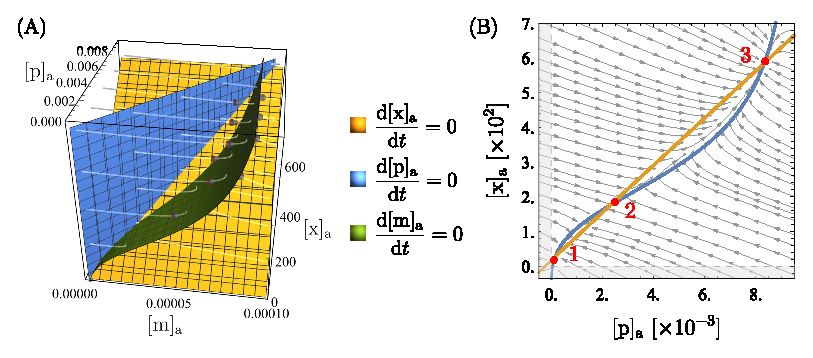
\includegraphics{media/Fig4_bistability.eps}
		\caption{{\bf Phase portraits showing bistability.}
			3D and 2D phase portraits for one set of parameters that leads to
			bistability. The parameter values are listed in
			Table~\ref{table1:nondim}. Note that all the concentrations
			($\n{[m]_a}, \n{[p]_a}, \n{[x]_a}$) are measured in units of
			$K_{\n{a}} = 5 \cdot 10^{4} \unit{nM}$. The surfaces in (A) and the
			curves in (B) are the nullclines of the state variables, and their
			intersection points, marked in red in (B), are the steady-state
			solutions of the system. The region shaded in gray in (B) leads to
			negative concentrations and is unphysical. A vector plot of (B) that
			also shows the magnitude of flow at each point can be found
			in~\nameref{S1_Text}.}
		\label{fig4:bistability}
	\end{figure}
	
	It is important to point out that, for a different set of parameters, the
	dynamics can be quite different. There are, for example, scenarios where the
	xanthosine kinetics are roughly as fast as the mRNA kinetics and the
	dynamics unfolds in two steps: first to the intersection of the mRNA and the
	xanthosine nullcline, then along that curve to the protein nullcline and
	thereby to a fixed point.
	
	A usual simplification with genetic circuits like this is to assume the mRNA
	concentration to be at steady-state, i.e., to write $\dd{\n{[m]_a}}{\tau}=0$
	and solve this for $\n{[m]_a}(\n{[p]_a},\n{[x]_a})$ to simplify the 3D to a
	2D system. This restricts the dynamics to the green surface in our plot, which
	is reasonable here because as explained above, the system first flows
	towards that surface before either the protein or the xanthosine concentration
	changes significantly. However, as already pointed out, this is different
	for other parameter values, and thus, this assumption does not hold in general.
	If the xanthosine dynamics are faster than the mRNA dynamics, the
	system first flows towards the xanthosine nullcline. In that case, forcing
	it onto the mRNA nullcline leads to significant changes in the dynamics.
	
	Nevertheless, the steady-state solutions and the qualitative features that
	we address in this paper remain the same. Because the 3D plots are rather
	hard to read, we will, in the following, make the compromise to show a 2D
	version of the phase portraits but ensure that all of our statements also
	hold true in 3D space. As explained above, it makes the most sense here to
	do this by setting $\dd{\n{[m]_a}}{\tau}=0$. The resulting equations can be
	found in~\nameref{S1_Text}. In particular, we define $\rho \defeq
	\frac{\rho_{\n{m}} \rho_{\n{p}}}{\gamma_{\n{mp}}}$ for everything that
	follows.
	
	\paragraph*{Bistability.} 
	We map the mRNA nullcline surface (green in Fig~\subref{fig4:bistability}{A}) onto a plane to show it as the 2D plot in Fig~\subref{fig4:bistability}{B}.
	From this 2D plot, it can clearly be seen
	that for the chosen parameters, there are three steady-state solutions.
	Because the system is restricted to the mRNA nullcline surface, these steady-state solutions are the same as those in the 3D plot
	($\dd{\n{[m]_a}}{\tau}=0$ on the nullcline and $\dd{\n{[p]_a}}{\tau}=0$,
	$\dd{\n{[x]_a}}{\tau}=0$ for the 2D fixed points). One can see from the
	vector field that the two outer fixed points (labeled 1 and 3) are stable and the
	middle one (labeled 2) is unstable and serves as a sort of ``switch-point''
	between the other two. This means that there are two stable states the cell
	can be in, one at high (point 3) and one at low (point 1) expression. As a
	result, there is bistability and the distribution of expression among cells
	can be bimodal, depending on initial conditions.
	
	The bistability corresponds to the experimental observations, so the model passes this
	sanity check. Furthermore, the xanthosine and protein concentrations at the
	upper fixed point have the expected order of magnitude: the xanthosine
	concentration is roughly $10-100 \unit{mM}$, and there are roughly $500$
	proteins, which is just a bit lower than what was measured for the number of
	Nup transporters~\cite{Li2014} which fulfill a similar purpose. We do not
	have well founded expectations for the other fixed points, so no comparison
	can be made here. Nevertheless, the orders of magnitude at the lower fixed
	point -- roughly $1-10 \unit{nM}$ of xanthosine and around $5$ proteins --
	seem quite reasonable. Note that $\n{[x]_a} \approx \n{[c]_a}$ at the
	lower fixed point because there is only weak accumulation due to Nup and a
	few XapB transporters.
	
	As already mentioned, we are working with one specific set of parameters
	here and we will now explain this choice of values. Firstly, they were
	picked roughly in the middle of the range that was estimated beforehand for this parameter (see Table~\ref{table1:nondim} and~\nameref{S1_Text}). Secondly, we
	chose parameters that allow clear bistability in the phase portraits as well as in the
	stochastic simulations (see later), which, of course, is not the case for any possible choice of parameters. Thirdly, by the corresponding choice of
	parameters it was ensured that the mRNA number per cell at the
	``switch-point'' is around 1: this is large enough to enable the system to
	clearly resolve the two stable fixed points (as we will see from the
	stochastic simulations later on), but is low enough to lead to mean mRNA
	numbers that are very reasonable (see~\cite{Milo2016} for the average mRNA
	numbers in bacterial cells). The protein and xanthosine
	concentrations followed from this, but with some variation in the parameters
	they could still be tuned to a certain extent.
	
	We point out that we have not observed any oscillations in the
	system. Intuitively, they might be expected when the XapA rate is
	significantly larger than the XapB rate, but it turns out that oscillations
	cannot be obtained. Why they do not occur can be understood when looking at the regions that
	are bounded by all three nullclines: on these boundaries, the streamlines
	point into the bounded regions, so deterministically, they serve as
	trapping regions from which the system cannot escape. Once inside, the only
	possible trajectory is non-oscillatory flow towards the stable fixed point.
	
	For a different set of parameters, the orders of magnitude in the plots and
	even the qualitative behavior can change. In the following, we will discuss
	some interesting features of the system that can be observed through the
	phase portraits. 
	
	\paragraph*{The extracellular xanthosine concentration.}
	The parameter that is the experimentally most easily tunable and
	biologically the most relevant is the extracellular xanthosine
	concentration. When it is increased in experiments, the cells go from (1.) all
	being in the low expression state to (2.) the population being in a mixed state with some cells in a low expression state and others in a high expression state (all-or-none phenomenon) and then to (3.) all being in the high
	expression state (see section ``experimental motivation''). If our model is correct, it should
	exhibit the same qualitative behavior. Indeed we find exactly this: as can
	be seen in Fig~\ref{fig5:extraxanth}, increasing $\n{[c]_a}$ makes the high
	stable fixed point appear and then, for even higher $\n{[c]_a}$, the lower
	one disappears. Thus, for low $\n{[c]_a}$ the only stable point of the system
	is at low expression, and for high $\n{[c]_a}$ there is only high
	expression. In between, there are two deterministically stable expression
	levels. Another means of visualizing this is with an bifurcation diagram, which we discuss in detail later.
	
	\begin{figure}%[h!]
		\centering
		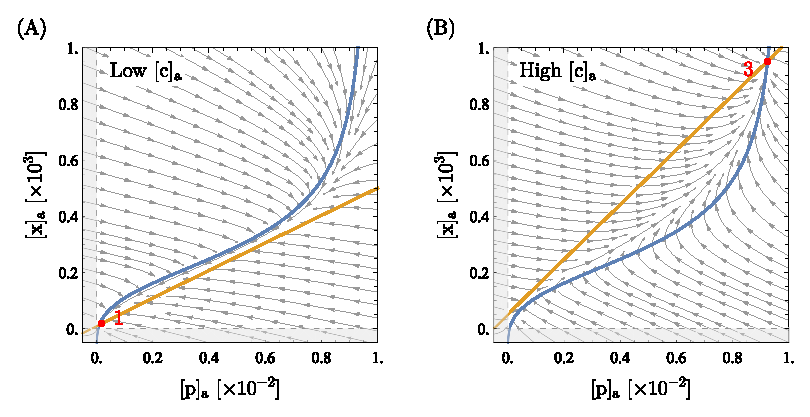
\includegraphics{media/Fig5_extraxanth.eps}
		\caption{{\bf Phase portraits for different extracellular xanthosine concentrations.}
			All parameters but $\n{[c]_a}$ are as presented in
			Table~\ref{table1:nondim}. The extracellular xanthosine
			concentration in these plots is $\n{[c]_a}=7$ in (A) and
			$\n{[c]_a}= 40$ in (B) (recall that $\n{[c]_{a}} \defeq
			\frac{c}{K_{\n{a}}}$ with $K_{\n{a}} = 5 \cdot 10^{-5} \unit{M}$,
			so $\n{[c]_a}$ is dimensionless).
			Tuning $\n{[c]_a}$ moves the orange line (xanthosine nullcline), but the blue curve (mRNA nullcline) is unchanged (see
			also~\nameref{S1_Text}). It can clearly be seen that in (A) there is
			only the lower fixed point (fixed point number 1), whereas in (B)
			there is only the upper one (fixed point number 3). In between lies
			the bistable case that was shown in Fig~\ref{fig4:bistability}.}
		\label{fig5:extraxanth}
	\end{figure}
	
	Furthermore, we found that in the absence of xanthosine, i.e., setting
	$\n{[c]_a}=0$ (not shown here), there are roughly 2-3 copies of XapA and XapB, which agrees very
	well with measurements, where around 2 copies per cell were
	found~\cite{Li2014}. In addition, the parameter $K_{\n{\chi A}}$
	(dissociation constant of xanthosine from active XapR) can be tuned such
	that the extracellular xanthosine concentration $\n{[c]_a}$ in the
	switching-regime is similar to that in the experiment. It was found that the
	cell only adapts at very high xanthosine concentrations of almost a
	millimolar~\cite{Norholm2001} which is not completely unexpected when
	recalling that for \emph{lac}, cells also limit themselves to glucose as
	long as possible. Interestingly, because there is no parameter other than
	$K_{\n{\chi A}}$ that tunes the critical value of $\n{[c]_a}$, this tells us
	that $K_{\n{\chi A}}$ is large as argued in the estimation of $K_{\n{\chi
			A}}$ in~\nameref{S1_Text}. Thus, we predict that the interaction between xanthosine and XapR
	should be weak.
	
	\paragraph*{The roles of XapA and XapB.}
	While it is clear that the bistability in the model system is due to the
	feedback loop from XapA and XapB, it is not intuitively clear if both XapA and XapB
	are necessary. The model implies that the bistability is due to XapB only. XapA
	is neither sufficient nor necessary and, within the estimated parameter
	regime, does not even have a significant influence on the system. This can
	be seen from the plots in Fig~\ref{fig6:xapAB}.
	Degradation of xanthosine by XapA lowers the xanthosine and protein concentration at the upper
	fixed point by a small amount and could, in principle, thereby make the
	high-expression solution vanish. For our choice of all other parameters,
	bistability only vanishes for $k_{\n{\alpha}} > 10^4$ which is far from what has been
	measured. However, a higher effective rate could, in principle, be achieved by
	different translation rates of XapA and XapB (see simplifications of the
	model in~\nameref{S1_Text}). Hence, we cannot exclude the possibility that
	XapA becomes so strong that it makes bistability impossible, but this is an
	extreme case. XapB, on the other hand, is essential; without it the system
	only has the one fixed point at low expression.\footnote{
		Seeger et.\ al.\cite{Seeger1995} observed that $\Delta xapB$ mutants could
		survive, but grew extremely slowly, with xanthosine as the only carbon
		source. This suggests that low-affinity
		import of xanthosine by NupC and NupG is sufficient to sustain slow growth,
		but insufficient to serve as a stand-in for XapB.
		Fig~\ref{fig6:xapAB} supports this supposition: in our model,
		with \textit{xapB} removed, the switch never activates and the cells are
		forced to survive with an extremely meager quantity of XapA to metabolize
		the abundant xanthosine.}
	
	\begin{figure}%[h!]
		\centering
		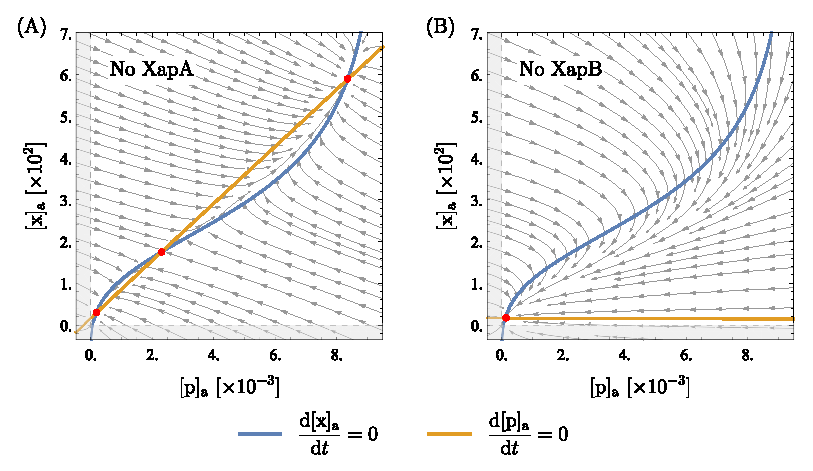
\includegraphics{media/Fig6_xapAB.eps}
		\caption{{\bf Phase portraits without XapA or XapB.}
			All parameters are as presented in Table~\ref{table1:nondim}. In
			(A), the XapA term was removed from the kinetic equations. In (B),
			the equations lack the two terms from XapB. These plots clearly show
			that XapA has almost no influence on the qualitative behavior of the
			system (i.e. bistability and the order of magnitudes), but XapB is
			the essential feature for bistability.}
		\label{fig6:xapAB}
	\end{figure}
	
	For a cell, the minimal effect of XapA on bistability is a useful feature: by coupling XapA and XapB on an
	operon, XapA is switched on and off together with XapB but it does not
	significantly disturb this adaptation mechanism, while its kinetic
	parameters and expression levels can be chosen 
	somewhat freely as necessary for metabolism. By
	having a membrane transporter gene on an operon whose expression is
	activated by the transporter substrate, the expression of a whole set of
	enzymes can be turned on and off depending on the presence of the substrate.
	It seems likely that this mechanism of short-term adaptation of a single cell to
	its environment may be used by cells for many metabolic processes.
	
	\paragraph*{The role of cooperativity.} 
	The model has two (putatively) cooperatively interacting binding sites for XapR on the
	\emph{xapAB} promoter and two cooperative binding sites on XapR for
	xanthosine. It is interesting to consider whether the cooperativity is
	a necessary feature for bistability. This question is motivated by the importance of
	cooperativity in ``typical'' genetic switches\cite{Gardner2000,Cherry2000}.
	
	If, as a purely theoretical consideration, we remove either the second
	xanthosine binding site on XapR or the second XapR binding site on the
	promoter, leaving cooperativity in only one component of the system,
	we find that the system still has a bistable parameter regime.
	However, this bistable parameter range is smaller than in the original
	model, which makes the system less stable: small stochastic fluctuations
	in the parameter values can collapse the system to monostability,
	possibly leaving it in the wrong state and without its ability to adapt.
	But only when the second binding site is removed in both places, leaving
	no cooperativity in the system, do we find that it is insufficiently non-linear to produce bistability. An example
	of the three scenarios (only cooperative XapR, only cooperative promoter, no cooperativity) can be seen in Fig~\ref{fig7:coop}. It follows that
	there need to be either two xanthosine binding sites on XapR or two XapR
	binding sites on the promoter (or both) in order to obtain a switch-like
	behavior. 
	
	\begin{figure}%[h!]
		\centering
		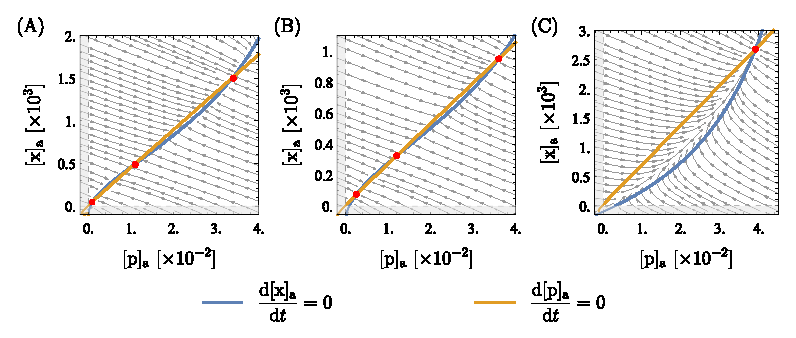
\includegraphics{media/Fig7_coop.eps}
		\caption{{\bf Phase portraits for less or no cooperativity.}
			Most parameters are as presented in Table~\ref{table1:nondim},
			changes are mentioned below. Fixed points are marked in red. In (A),
			there is only one xanthosine binding site on XapR and everything
			unchanged for the XapR-promoter binding. Two parameters are changed:
			$\rho = 0.07$ and $\n{[c]_a} = 6$. This is necessary to compensate
			for the weaker induction such that the system is bistable. In (B),
			there is only one XapR binding site on the promoter and everything
			is unchanged for the xanthosine-XapR binding. Two parameters are
			changed: $\rho = 0.13$ and $\n{[c]_a} = 3$. In (C), there is only
			one xanthosine binding site on XapR and also only one XapR binding
			site on the the promoter. Two parameters are changed: $\rho = 0.1$
			and $\n{[XapR]_R} = 5$. Whereas bistability is retained in (A) and
			(B), it cannot be obtained anymore in (C).}
		\label{fig7:coop}
	\end{figure}
	
	One can also ask how much cooperative interaction is needed between the two
	binding sites. For the promoter, the amount of cooperativity is given by $\Delta E_{\n{coop}}$ in
	our model, and we find that setting $\Delta E_{\n{coop}} = 0$ has almost no
	influence on the phase diagrams. For XapR, we cannot test how much interaction is needed: the two binding sites interact
	indirectly, because the active state is much likelier if two xanthosine
	molecules are bound, and thus there is no continuous tuning parameter for the cooperative interaction
	like $\Delta E_{\n{coop}}$ in the case of the promoter.
	
	Note that we are not writing Hill equations and measuring cooperativity in
	terms of the Hill coefficient. If Hill equations were to be used for the
	modeling, the Hill coefficient could have values between 1 and 2, which
	would yield bistability for large enough values, but not for lower ones.
	This could be investigated more rigorously similar to the analysis of a
	simple genetic switch in~\cite{Cherry2000}. However, we refrain from looking
	for a minimal Hill coefficient in our system, because we do not find this
	very insightful. Hill equations only describe some specific limit cases of cooperative systems, but for example do not account for interaction energies and assume the partially bound states (e.g. only one XapR bound to the promoter) to never be populated.
	We suggest that cooperativity should be explored more in-depth and a more
	rigorous analysis of the role of cooperativity in simple genetic switches
	should be done before returning to more complex systems like this one.
	
	\subsection*{Stochastic simulations}
	Stochastic simulations of the full 3-dimensional system of mRNA, protein,
	and xanthosine were run for comparison with the deterministic results.
	In~\nameref{S1_Text}, we present the underlying chemical master equation of
	the system. Because of the two different fixed points at low and high
	expression, the protein copy numbers in the problem vary from less than
	five to several thousand. Even worse, xanthosine copy numbers may range
	as high as $10^7$ at the high expression fixed point. For such large
	copy numbers, the number of reaction firings that must be simulated with
	Gillespie's classical algorithm leads to an impractical computational
	cost. This would make Gillespie's \texttau-leap algorithm ideal for the high
	expression state. On the other hand, \texttau-leaping cannot be used for
	the small protein copy numbers in the low expression state, or the mRNA
	copy number which remains of order ten or less in both states. For
	these reasons, we chose to work with the algorithm described
	in~\cite{Cao2006}, a hybrid form between Gillespie's classical and his
	\texttau-leap algorithm. We gratefully worked with the Python implementation
	of this algorithm in \emph{StochPy}, version 2.3~\cite{Maarleveld2015}.
	
	Note that we neglect stochastic fluctuations in any of our parameters, in particular in the XapR copy number. The latter is on the order of 10, but because of the long life span and rare expression of proteins like XapR, we expect the influence of the simplification on our results to be rather small. Nevertheless, the overall stochastic fluctuations are expected to be larger in the real system than in our simulations.
	
	\paragraph*{Bimodality and the extracellular xanthosine concentration.}
	The stochastic approach results in the same bimodal distributions that were already
	seen in the deterministic investigation and experimental studies.
	Fig~\ref{fig8:stochC} shows the distribution of protein expression found in
	the simulations for different values of the extracellular xanthosine
	concentration. The parameters that were used are the same as in the previous
	section (listed in Table~\ref{table1:nondim}). However, we also find good agreement of the simulations and the deterministic results for other sets of parameters. To obtain the distributions,
	we ran the simulation 5000 times for a simulated time of $10^6 \unit{s}$
	each and started at an mRNA, protein and intracellular xanthosine count of 0.
	
	\begin{figure}%[h!]
		\centering
		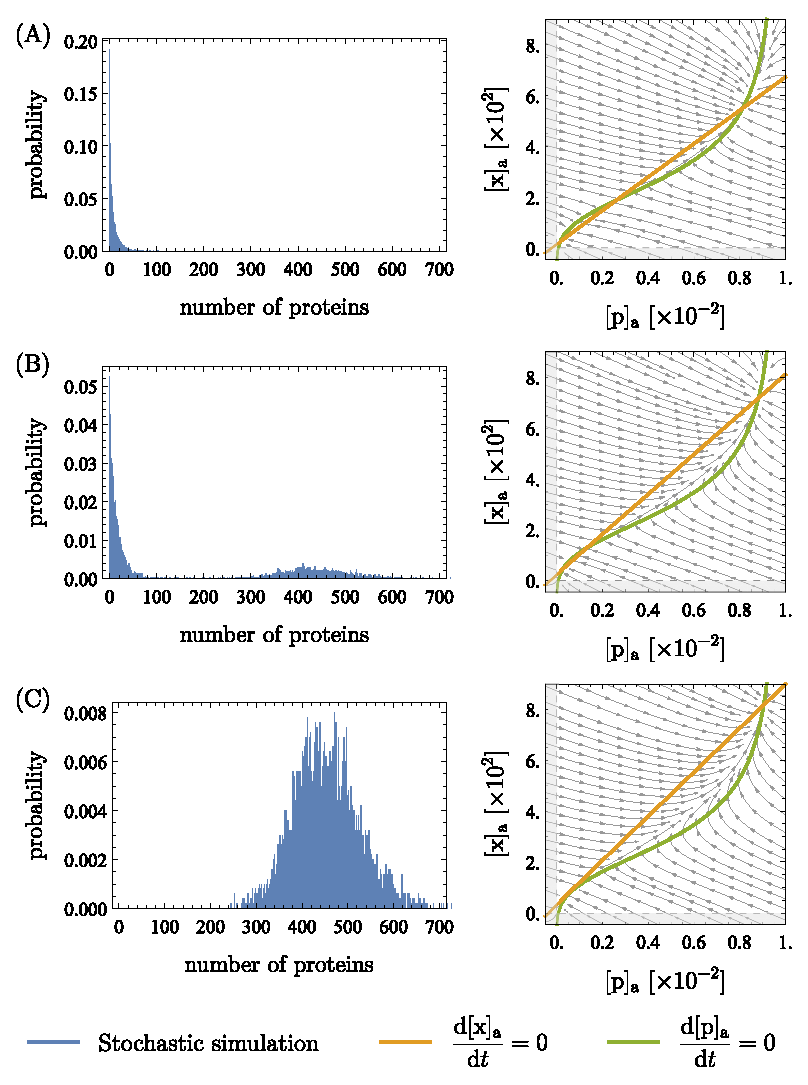
\includegraphics{media/Fig8_distribution.eps}
		\caption{{\bf Distributions from stochastic simulations and the corresponding phase portraits.}
			Apart from $\n{[c]_a}$, the parameters are the same as in
			Table~\ref{table1:nondim}. For the distributions, the simulations
			were run 5000 times for $10^6 \unit{s}$ each (simulated time) and
			started at a mRNA, protein and intracellular xanthosine count of 0.
			We show the two cases of unimodality (low expression in (A) and high
			expression in (C)) as well as the case of bimodality in (B). The
			values of $\n{[c]_a}$ are 12 in (A), 18.5 in (B), and 25 in (C)
			(recall that $\n{[c]_{a}} \defeq
			\frac{c}{K_{\n{a}}}$ with $K_{\n{a}} = 5 \cdot 10^{-5} \unit{M}$,
			so $\n{[c]_a}$ is dimensionless). The output from the stochastic simulations
			is in good agreement with the concentrations at the fixed points in
			the deterministic phase portraits.}
		\label{fig8:stochC}
	\end{figure}
	
	The results agree very well with the deterministic fixed points and
	experiments: the mean numbers of mRNA, protein, and xanthosine in the
	stochastic results are as predicted from the phase portraits. It does,
	however, become clear that the phase portraits do not tell whether the cells
	will actually populate both the high and the low expression state,
	because they do not show the effective barrier height between the two states.
	In Fig~\subref{fig8:stochC}{(A)}, a deterministically bistable scenario is shown where the cells never switched to the high
	expression state during the run time of our simulations. This result
	implies that bistability, characterized by two separate
	\emph{stable} steady-states, largely persists even in the presence
	of stochastic fluctuations, suggesting that the deterministic
	picture is remarkably effective. In other words,
	the fact that bimodality only occurs with some fine tuning of
	parameters means that the circuit is a strong switch and the
	deterministic picture is sufficient except in a small region of
	parameter space. Whether or not the system is actually in that
	region of parameter space remains a question for future experiments.

	To elaborate on the preceeding statements,
	we found that the two lower fixed points (marked as 1 and 2 in
	Fig~\ref{fig4:bistability}) need to be very close like in
	Fig~\subref{fig8:stochC}{(B)} to give bimodality. For lower $\n{[c]_a}$,
	meaning larger difference between the concentrations at the first and second fixed point,
	almost no switching was observed. Of course, switching is also a matter of the
	waiting time and stochastic effects: if one waits for long enough, it
	should eventually occur. However, switching times of more than several hours
	are not at the center of this investigation and would mean that switching is
	extremely unlikely. There are two aspects that become relevant in this
	context that we neglect in our analysis but briefly mention here:
	transcription and translation bursts lead to higher stochasticity and cell
	division leads to some discontinuity in the process. The effect of bursts is addressed in~\nameref{S1_Text}.
	
	Note that while the deterministic analysis assumes the variables to be
	continuous, the simulations work with discrete numbers of mRNA, protein, and
	xanthosine. This per se is no problem, because the deterministic analysis
	describes the mean values and the simulation fluctuates around this mean.
	However, if the mRNA number of the third (high) fixed point is so low that stochastic fluctuations are larger than the difference in concentrations between the first and the second fixed point, the
	system may not be able to resolve the two points anymore. The tolerance to this is surprisingly large, though: In Fig~\ref{fig8:stochC}, the distance between the first and the third fixed point is around 3 mRNA molecules. While this is around the size of the fluctuations in Fig~\ref{fig8:stochC}, the latter become as large as 10 mRNA molecules when bursts are included in the simulation (see~\nameref{S1_Text}) and yet, the system is able to resolve the fixed points very well.
	
	\paragraph*{Time evolution and adaptation times.}
	Fig~\subref{fig9:StochT}{A} shows the time evolution of the protein concentration for one typical run of the simulation.
	Again, the simulation was started with a mRNA, protein and intracellular
	xanthosine count of 0 and was run for a simulated time of $5 \cdot 10^5
	\unit{s}$. In this specific example, the fixed point was reached after roughly $1.5 \cdot 10^5
	\unit{s}$ (adaptation time).
	This time varies: Fig~\subref{fig9:StochT}{B} shows the distribution
	of adaptation times from 1000 runs of the simulation.
	In both figures, the trajectory obtained from
	integrating the deterministic system is shown for comparison. It
	clearly agrees well with the simulation on average.
	
	\begin{figure}%[h!]
		\centering
		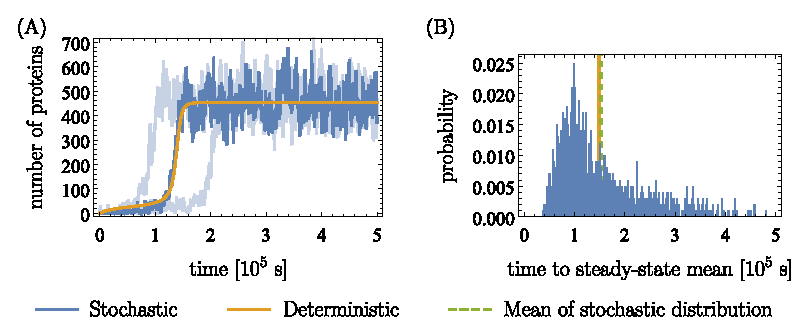
\includegraphics{media/Fig9_evolution.eps}
		\caption{{\bf Stochastic and deterministic time evolution of protein (XapA/XapB) and adaptation time.}
			(A) Shown in blue is the result from one typical run of the stochastic simulation, and in orange the trajectory obtained from solving the deterministic ODE's. In light blue, two more extreme runs of the simulation are shown for comparison. The simulation was run for $5 \cdot 10^5 \unit{s}$ each and started
			at an mRNA, protein and intracellular xanthosine count of 0. The parameters that were used are the same as in
			Table~\ref{table1:nondim}, the only exception being the
			extracellular xanthosine concentration, which was chosen to be
			$\n{[c]_a} = 25$ (recall $\n{[c]_{a}} \defeq \frac{c}{K_{\n{a}}}$,
			$K_{\n{a}} = 5 \cdot 10^{-5} \unit{M}$) just as in
			Fig~\subref{fig8:stochC}{(C)}.
			(B) In blue we plot the waiting time distribution for 1000
			runs of the simulation (same conditions as (A)) to reach
			the steady-state mean.
			We define this time as the elapsed time when the protein
			copy number first reaches 90\% of its value at the upper
			fixed point.
			To better visualize the bulk of the distribution, we
			excluded from the plot $\sim10$ runs with adaptation times
			larger than $6 \cdot 10^5 \unit{s}$.
			The green dashed line indicates the mean of the blue distribution.
			The orange line shows the corresponding deterministic time.
			}
		\label{fig9:StochT}
	\end{figure}
	
	Comparing this to experimentally expected timescales is difficult,
	because the adaptation time strongly depends on the extracellular xanthosine
	concentration. Experiments were always stopped after a few hours, and in
	this time, the cell population might not reach its steady-state expression
	distribution. Hence, the distribution could be bimodal when the experiment
	is stopped but become unimodal after further waiting. That way,
	extracellular xanthosine concentrations that are too high for deterministic
	bistability could lead to experimental bimodality if the experiment is
	stopped too early. In this case, the observed timescales would be
	shorter, which makes the comparison to our simulations even harder. Thus, we
	cannot say if it is problematic that the $10^5 \unit{s}$ is larger than what
	was found in the experiment. 
	
	Nevertheless, we do warn the reader that the timescales in the simulations and even more so in the deterministic system
	should be taken with reservation. Fluctuations in the parameters are not considered here, and neither are cell divisions or the burstiness of transcription and translation. This means
	that stochasticity may be larger in the real system which should have an
	influence on the timescales and may shorten the time until the fixed point is reached. However, including transcriptional bursts in the stochastic simulation changes little in the output: the qualitative behavior remains the same but fluctuations around the mean as well as in the adaptation time become larger and bimodality already occurs at lower $\mathrm{[c]_a}$ (see~\nameref{S1_Text}). Still, the fact that there are no big changes shows that the system is stable to stochastic perturbations and our particular assumptions should not be too significant.
	
	Of course, the system moves to its mean steady-state much faster when the extracellular xanthosine concentration is further away from the bimodal regime (in analogy to a ``critical point''). 
	Note that it could well be that in reality, the extracellular xanthosine concentration is high enough to be in the regime where there only is the upper fixed point and thus no bistability or even bimodality. As the system reaches its mean steady-state faster in that regime, the bacteria could adapt more quickly.
	
	\paragraph*{Bifurcation diagram and hysteresis.} 
	In Figs~\ref{fig8:stochC} and~\ref{fig9:StochT}, the simulations were started at initial intracellular concentrations of 0 to investigate what happens if xanthosine is suddenly added to the cell's environment. We can now ask the opposite question: what happens when xanthosine is removed from the extracellular environment? To answer this, the simulation was started with initially fully	induced cells, i.e. at the mRNA, protein and intracellular xanthosine counts of the high fixed point in the corresponding phase portrait. 
	
	The distributions we obtained can be found in~\nameref{S1_Text}. Here, we instead present the results in the form of a bifurcation diagram in Fig~\ref{fig10:Bifurcation}. In blue, the positions of the deterministic fixed points for the corresponding extracellular xanthosine concentration are shown. As explained before, there is only one fixed point for low and high values of $\mathrm{[c]_a}$, but in between, there are three. In yellow and orange, the results from the stochastic simulation are shown, where the mean of each distribution was taken. For the orange points, the simulation was started at $\mathrm{[m]_a}=\mathrm{[p]_a}=\mathrm{[x]_a}=0$, leading to the distributions in Fig~\ref{fig8:stochC}. In contrast, the yellow points result from starting the simulation at the $\mathrm{[m]_a}$, $\mathrm{[p]_a}$, and $\mathrm{[x]_a}$ values of the high fixed point. Note that by taking the mean of each distribution, we hide the feature of bimodality. For that reason, we additionally show the approximate position of the two peaks in the bimodal distribution. We do this by estimating the position of the minimum between the two peaks of the distribution, splitting it into two parts there, and calculating the mean of each of the parts. Also note that it suffices to show the bifurcation diagram in one dimension (here protein concentration) because this uniquely determines the fixed points (recall from Fig~\ref{fig4:bistability}, the fixed points are unique points in the 3D system).
	
	\begin{figure}%[h!]
		\centering
		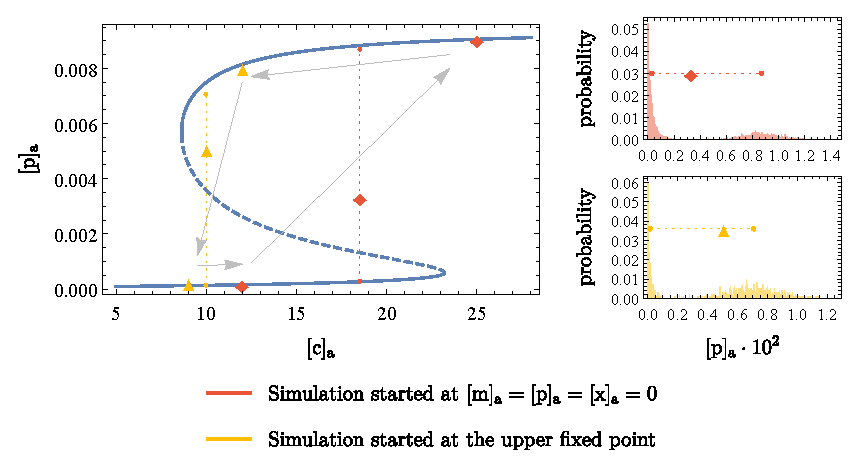
\includegraphics{media/Fig10_bifurcation.eps}
		\caption{{\bf Bifurcation diagram showing the hysteresis loop in the stochastic system.}
			The blue line shows the positions of the deterministic fixed
			points, while the dashed line indicates the instability of
			the middle one. The orange and yellow points show the mean
			of the stochastic simulations when started at zero and at
			the high fixed point, respectively. The positions of the two
			peaks in the bimodal distributions are indicated by smaller
			points, connected by dotted lines. To make this clearer, the
			bimodal distributions themselves are shown in a light color (in a smoothed form). The arrows illustrate the
			hysteresis loop in the stochastic simulations.
			}
		\label{fig10:Bifurcation}
	\end{figure}
		
	The figure clearly shows the hysteresis in the system: there exist extracellular xanthosine concentrations where
	initially uninduced cells remain uninduced and initially induced cells remain induced. Only when the second and the third fixed point are very close can initially induced cells ``switch off'' to the uninduced state. This
	behavior is symmetric to the ``switching on'' in the previous paragraphs. The arrows in Fig~\ref{fig10:Bifurcation} indicate the hysteresis loop.
	
	In other words, cells only change their metabolism to xanthosine if
	enough of the latter is around, but after they have switched, this metabolic
	state is stable even if the xanthosine concentration decreases to a certain
	extent. This stability explains what was observed by Novick and
	Weiner~\cite{Novick1957} for the \emph{lac} operon: when induced cells were
	transferred into lower concentrations of lactose, they remained induced,
	even though uninduced cells could not become induced at these
	concentrations.
	
	In addition to the hysteresis, Fig~\ref{fig10:Bifurcation} also illustrates the astonishingly good agreement of the stochastic simulation and the deterministic results, despite having copy numbers below 10 in some cases. Although one should be cautious about this because of higher stochasticity in the real biological system (addressed above), the result does show that the switch-like feature in the circuit is strong and stable.
	
	
	\section*{Conclusion}
	Here, we propose a simple model for genetic circuits containing
	a membrane transporter whose gene expression is, directly or indirectly,
	activated by its substrate. We have shown that such a system can be bistable
	and thus work as a genetic switch which reacts to the extracellular
	concentration of the relevant metabolite. This switch has very useful
	biological features. First, coupling of the transporter with, for example, an
	enzyme which metabolizes the transporter substrate creates a genetic switch that enables short-term
	adaptation of the cell's metabolism to its environment. Second, the switch
	is stabilized by hysteresis effects when the extracellular substrate
	concentration decreases, which explains previous experimental findings.
	Furthermore, our simulations show that the switch-like behavior is very robust. 
	
	However, we have found that no bistability can emerge from the genetic circuit unless
	at least one component has two binding sites for its activator. Additional
	binding sites or cooperativity seem to increase the stability of the switch.
	In addition, simply knowing the experimental switching concentration of
	xanthosine permits us, for example, to infer the approximate value of the
	dissociation constant between the transcription factor XapR and the inducer
	xanthosine. The value we infer is roughly one to two orders of magnitude
	larger than what has been measured for LacI and
	IPTG~\cite{RazoMejia2018}, meaning the interaction of XapR and
	xanthosine is rather weak.
	
	Phase diagrams, showing for which parameters the system is bistable and for
	which there is only the lower or the upper stable fixed point, could be
	calculated from arguments made in~\cite{Cherry2000}. However, the
	simulations showed that in the deterministically bistable regime, which fixed point(s) the system occupies is dependent on initial conditions, which is why we have refrained from showing such phase
	diagrams. Furthermore, the timescales in the problem could be investigated
	more thoroughly, for example the dependence of the switching time on
	$\n{[c]_a}$, but such an analysis should probably account for	cell divisions and fluctuations in the parameters, which is not straightforward. Lastly, it could be interesting to investigate the magnitude of the fluctuations around the fixed point away from and near the bifurcations in $\mathrm{[c]_a}$.
	
	Despite the small copy numbers at the lower fixed point, the stochastic simulations are in excellent agreement with deterministic predictions. All model parameters could be reasonably estimated despite the paucity of
	experimental knowledge about the model system. The concentrations of mRNA, protein, and xanthosine at the fixed points as well as all qualitative features are as expected from similar systems and the few experiments on the \emph{xap} circuit. These points suggest that the model captures the relevant components of the system correctly and is able to describe its
	dynamics. 
	The modeling results let us, to some extent, understand how the biological system can achieve its function. By keeping the model as minimal as possible, but still modeling every part explicitly with an appropriate complexity, we can investigate the interesting features while still being able to understand the influence of all parameters and their interplay intuitively.
		
	With the framework given in this text, it
	should be straightforward to model other promoters, regulatory pathways or
	enzymes and thereby adapt the model to other genes and metabolites. Examples
	include \emph{lac}, \emph{ara}, and \emph{xyl}, but we suspect that many if
	not most metabolic processes involve the adaptation mechanism that we have
	investigated here, and that much can be understood about them through our
	model. This apparent success demonstrates once more that even for broadly
	unknown systems, rigorous physical modeling can potentially offer an
	efficient way to gain a very thorough understanding of the behavior of the
	system. 
	
	
	\section*{Supporting information}
	\paragraph*{S1 Text.}
	\label{S1_Text}
	{\bf The aforementioned further information.} Discussion of simplifications
	in the model, parameter estimation, elaborations on the results, and the
	chemical master equation of this circuit. Experimental materials and methods.
	
	\section*{Acknowledgments}
	We thank Jane Kondev and Jin Wang for interesting discussions, Patrick Lenggenhager for his help with \emph{Mathematica} issues, and Nigel Orme for assistance with illustrations.
	Portions of the experiments reported here were carried out at the
	Physiology Course at the Marine Biological Laboratory in Woods
	Hole, MA, operated by the University of Chicago.
	This work was supported by 1R35 GM118043-01 Maximizing Investigators'
	Research Award (MIRA) (to R.P.), and the Werner Siemens Foundation
	through the Swiss Study Foundation (K.S.L.). This material is based upon
	work supported by the National Science Foundation Graduate Research
	Fellowship under Grant No.\ DGE-1745301 (M.J.M.).
	
	\nolinenumbers
	
	% Either type in your references using
	% \begin{thebibliography}{}
	% \bibitem{}
	% Text
	% \end{thebibliography}
	%
	% or
	%
	% Compile your BiBTeX database using our plos2015.bst
	% style file and paste the contents of your .bbl file
	% here. See http://journals.plos.org/plosone/s/latex for 
	% step-by-step instructions.
	
	\begin{thebibliography}{10}
		
		\bibitem{Jacob1961}
		Jacob F, Monod J.
		\newblock Genetic regulatory mechanisms in the synthesis of proteins.
		\newblock Journal of Molecular Biology. 1961;3(3):318--356.
		
		\bibitem{Gardner2000}
		Gardner TS, Cantor CR, Collins JJ.
		\newblock Construction of a genetic toggle switch in \emph{Escherichia coli}.
		\newblock Nature. 2000;403:339.
		
		\bibitem{Wolf1998}
		Wolf DM, Eeckman FH.
		\newblock On the Relationship between Genomic Regulatory Element Organization
		and Gene Regulatory Dynamics.
		\newblock Journal of Theoretical Biology. 1998;195(2):167 -- 186.
		\newblock doi:{https://doi.org/10.1006/jtbi.1998.0790}.

		\bibitem{Wong1997}
		Wong P, Gladney S, Keasling JD.
		\newblock Mathematical Model of the \textit{lac} Operon: Inducer Exclusion,
		Catabolite Repression, and Diauxic Growth on Glucose and Lactose.
		\newblock Biotechnology Progress. 1997;13(2):132 -- 143.
		\newblock doi:{https://doi.org/10.1021/bp970003o}.

		\bibitem{Novick1957}
		Novick A, Weiner M.
		\newblock Enzyme induction as an all-or-none phenomenon.
		\newblock Proceedings of the National Academy of Sciences of the United States
		of America. 1957;43(16590055):553--566.
		
		\bibitem{Santillan2008}
		Santillán M, Mackey MC.
		\newblock Quantitative approaches to the study of bistability in the \emph{lac}
		operon of \emph{Escherichia coli}.
		\newblock Journal of The Royal Society Interface. 2008;5(suppl\_1):S29--S39.
		\newblock doi:{10.1098/rsif.2008.0086.focus}.
		
		\bibitem{Narang2008}
		Narang A, Pilyugin SS.
		\newblock Bistability of the lac Operon During Growth of Escherichia coli on
		Lactose and Lactose + Glucose.
		\newblock Bulletin of Mathematical Biology. 2008;70(4):1032--1064.
		
		\bibitem{Choi2008}
		Choi PJ, Cai L, Frieda K, Xie XS.
		\newblock A Stochastic Single-Molecule Event Triggers Phenotype Switching of a
		Bacterial Cell.
		\newblock Science. 2008;322(5900):442--446.
		\newblock doi:{10.1126/science.1161427}.
		
		\bibitem{Ozbudak2004}
		Ozbudak EM, Thattai M, Lim HN, Shraiman BI, van Oudenaarden A.
		\newblock Multistability in the lactose utilization network of
		\emph{Escherichia coli}.
		\newblock Nature. 2004;427:737.
		
		\bibitem{Fritz2014}
		Fritz G, Megerle JA, Westermayer SA, Brick D, Heermann R, Jung K, et~al.
		\newblock Single Cell Kinetics of Phenotypic Switching in the Arabinose
		Utilization System of E. coli.
		\newblock PLOS ONE. 2014;9(2):e89532.
		\newblock doi:{10.1371/journal.pone.0089532}.
		
		\bibitem{Jenkins2017}
		Jenkins A, Macauley M.
		\newblock Bistability and Asynchrony in a Boolean Model of the l-arabinose
		Operon in Escherichia coli.
		\newblock Bulletin of Mathematical Biology. 2017;79(8):1778--1795.
		
		\bibitem{Siegele1997}
		Siegele DA, Hu JC.
		\newblock Gene expression from plasmids containing the araBAD promoter at
		subsaturating inducer concentrations represents mixed populations.
		\newblock Proceedings of the National Academy of Sciences of the United States
		of America. 1997;94(9223333):8168--8172.
		
		\bibitem{Bae2010}
		Bae JS, Kim TH, Kim MY, Park JM, Ahn YH.
		\newblock Transcriptional Regulation of Glucose Sensors in Pancreatic
		beta-Cells and Liver: An Update.
		\newblock Sensors. 2010;10(5):5031–5053.
		\newblock doi:{10.3390/s100505031}.
		
		\bibitem{Tiedge1991}
		Tiedge M, Lenzen S.
		\newblock Regulation of glucokinase and GLUT-2 glucose-transporter gene
		expression in pancreatic beta-cells.
		\newblock The Biochemical journal. 1991;279 (Pt 3)(1953686):899--901.
		
		\bibitem{Song1997}
		Song S, Park C.
		\newblock Organization and regulation of the D-xylose operons in \emph{Escherichia
		coli} K-12: XylR acts as a transcriptional activator.
		\newblock Journal of Bacteriology. 1997;179(22):7025--7032.
		\newblock doi:{10.1128/jb.179.22.7025-7032.1997}.
		
		\bibitem{Schmidt2015}
		Schmidt A, Kochanowski K, Vedelaar S, Ahrné E, Volkmer B, Callipo L, et~al.
		\newblock The quantitative and condition-dependent \emph{Escherichia coli} proteome.
		\newblock Nature Biotechnology. 2015;34:104.
		
		\bibitem{Buxton1980}
		Buxton RS, Hammer-Jespersen K, Valentin-Hansen P.
		\newblock A second purine nucleoside phosphorylase in \emph{Escherichia coli}
		K-12.
		\newblock Molecular and General Genetics MGG. 1980;179(2):331--340.
		
		\bibitem{Hammer-Jespersen1980}
		Hammer-Jespersen K, Buxton RS, Hansen TD.
		\newblock A second purine nucleoside phosphorylase in \emph{Escherichia coli}
		K-12.
		\newblock Molecular and General Genetics MGG. 1980;179(2):341--348.
		
		\bibitem{Seeger1995}
		Seeger C, Poulsen C, Dandanell G.
		\newblock Identification and characterization of genes (xapA, xapB, and xapR)
		involved in xanthosine catabolism in \emph{Escherichia coli}.
		\newblock Journal of bacteriology. 1995;177(7559336):5506--5516.
		
		\bibitem{Joergensen1999}
		Jorgensen C, Dandanell G.
		\newblock Isolation and characterization of mutations in the \emph{Escherichia
			coli} regulatory protein XapR.
		\newblock Journal of bacteriology. 1999;181(10400599):4397--4403.
		
		\bibitem{Norholm2001}
		Norholm MH, Dandanell G.
		\newblock Specificity and topology of the \emph{Escherichia coli} xanthosine
		permease, a representative of the NHS subfamily of the major facilitator
		superfamily.
		\newblock Journal of bacteriology. 2001;183(11466294):4900--4904.
		
		\bibitem{Garcia2011}
		Garcia HG, Phillips R.
		\newblock Quantitative dissection of the simple repression input-output
		function.
		\newblock Proceedings of the National Academy of Sciences of the United States
		of America. 2011;108 29:12173--8.
		
		\bibitem{RazoMejia2018}
		Razo-Mejia M, Barnes SL, Belliveau NM, Chure G, Einav T, Lewis M, et~al.
		\newblock Tuning Transcriptional Regulation through Signaling: A Predictive
		Theory of Allosteric Induction.
		\newblock Cell Systems. 2018;6(4):456 -- 469.e10.
		\newblock doi:{https://doi.org/10.1016/j.cels.2018.02.004}.
		
		\bibitem{Chure2019}
		Chure G, Kaczmarek ZA, Phillips R.
		\newblock Physiological Adaptability and Parametric Versatility in a Simple
		Genetic Circuit.
		\newblock bioRxiv. 2019;doi:{10.1101/2019.12.19.878462}.
		
		\bibitem{Marzen2013}
		Marzen S, Garcia HG, Phillips R.
		\newblock Statistical Mechanics of Monod--Wyman--Changeux (MWC) Models.
		\newblock Journal of Molecular Biology. 2013;425(9):1433 -- 1460.
		\newblock doi:{https://doi.org/10.1016/j.jmb.2013.03.013}.
		
		\bibitem{Kaback2015}
		Kaback HR.
		\newblock A chemiosmotic mechanism of symport.
		\newblock Proceedings of the National Academy of Sciences.
		2015;112(5):1259--1264.
		\newblock doi:{10.1073/pnas.1419325112}.
		
		\bibitem{Li2014}
		Li GW, Burkhardt D, Gross C, Weissman J.
		\newblock Quantifying Absolute Protein Synthesis Rates Reveals Principles
		Underlying Allocation of Cellular Resources.
		\newblock Cell. 2014;157(3):624 -- 635.
		\newblock doi:{https://doi.org/10.1016/j.cell.2014.02.033}.
		
		\bibitem{Milo2016}
		Milo R, Phillips R.
		\newblock In: Cell biology by the numbers. Garland Science. 2016; 217.
		
		\bibitem{Cherry2000}
		Cherry JL, Adler FR.
		\newblock How to make a Biological Switch.
		\newblock Journal of Theoretical Biology. 2000;203(2):117--133.
		
		\bibitem{Cao2006}
		Cao Y, Gillespie DT, Petzold LR.
		\newblock Efficient step size selection for the tau-leaping simulation method.
		\newblock J Chem Phys. 2006;124(4):044109.
		\newblock doi:{10.1063/1.2159468}.
		
		\bibitem{Maarleveld2015}
		Maarleveld TR, Olivier BG, Bruggeman FJ. StochPy, Stochastic Modeling in
		Python. 2015.
		\newblock Available from: \url{http://stochpy.sourceforge.net/}.
		
	\end{thebibliography}
	
\end{document}